\documentclass{beamer}

\usepackage[utf8]{inputenc}
\usepackage[T1]{fontenc}
\usepackage{amsmath}
\usepackage{bm}

\usepackage{tabularx}
\usepackage{graphicx}
\usepackage{epstopdf}

\graphicspath{{../../images/}}

\usetheme{Madrid}
\usebeamercolor{sidebartab}
\usefonttheme{professionalfonts}


\title[M.Sc. Thesis 2015]{Spatial Summarization of Image Collections}
\author{Diego A. Ballesteros Villamizar}
\institute[ETHZ]{ETH Zürich}
\date{December 2nd, 2015}

\DeclareMathOperator*{\argmin}{argmin}
\DeclareMathOperator*{\argmax}{argmax}

\AtBeginSection[]
{
  \begin{frame}<beamer>
    \frametitle{Outline}
    \tableofcontents[currentsection]
  \end{frame}
}

\begin{document}

  \begin{frame}
    \titlepage
  \end{frame}
  
  \section{FLID Results}
  
  \begin{frame}{Recap}
    \begin{table}
      \begin{tabularx}{0.7\textwidth}{X|c|c|c|c}
        Model         & $Acc$ & $\sigma_{Acc}$ & $MRR$ & $\sigma_{MRR}$ \\
        \hline
        Modular       & 16.42 & 2.42           & 44.47 & 1.40 \\
        FLID ($d=2$)  & 18.95 & 2.60           & 45.35 & 1.64 \\
        FLID ($d=5$)  & 24.50 & 4.14           & 48.73 & 2.85 \\
        FLID ($d=10$) & 26.32 & 3.35           & 50.00 & 1.92 \\
        FLID ($d=20$) & 26.75 & 2.18           & 50.20 & 1.53 \\ 
      \end{tabularx}
    \end{table}
  \end{frame}
  
  \begin{frame}{Choosing d}
    \begin{figure}
      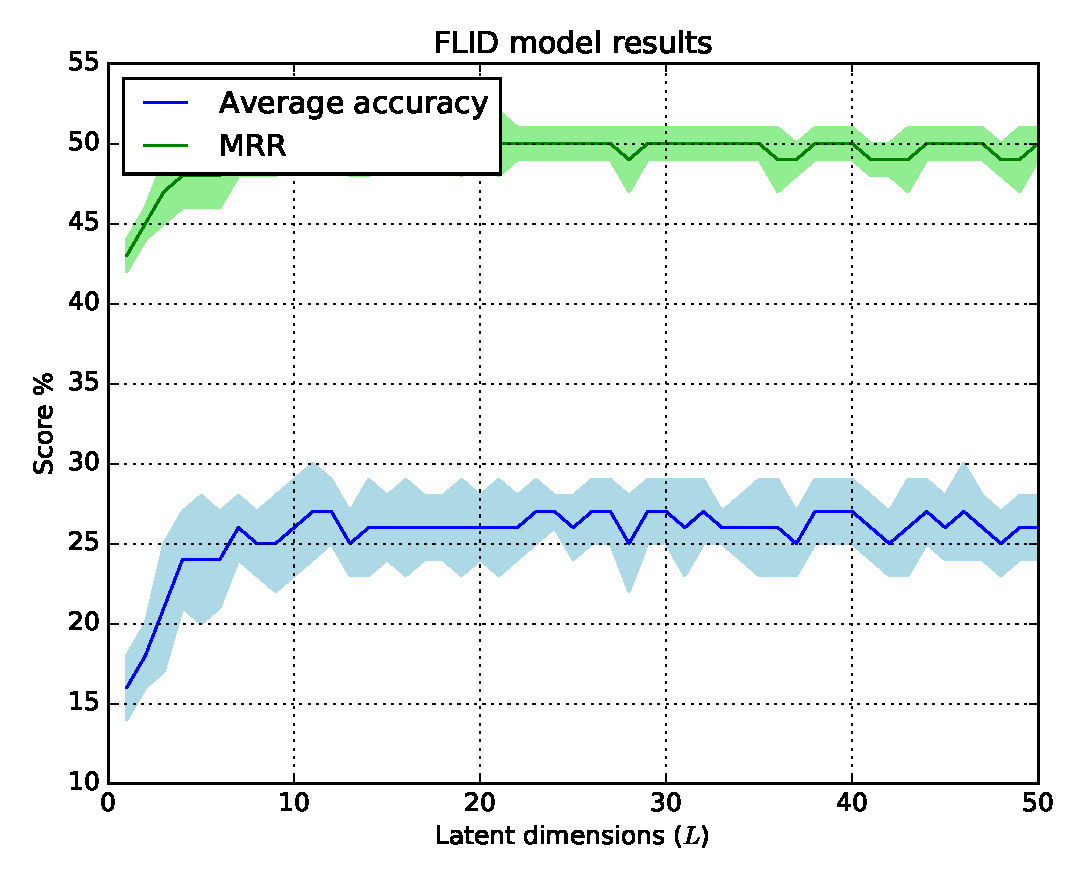
\includegraphics[width=0.7\textwidth]{submodular_score}
    \end{figure}
  \end{frame}
  
  \begin{frame}{Diversity Encoding ($d=2$)}
    \begin{figure}
      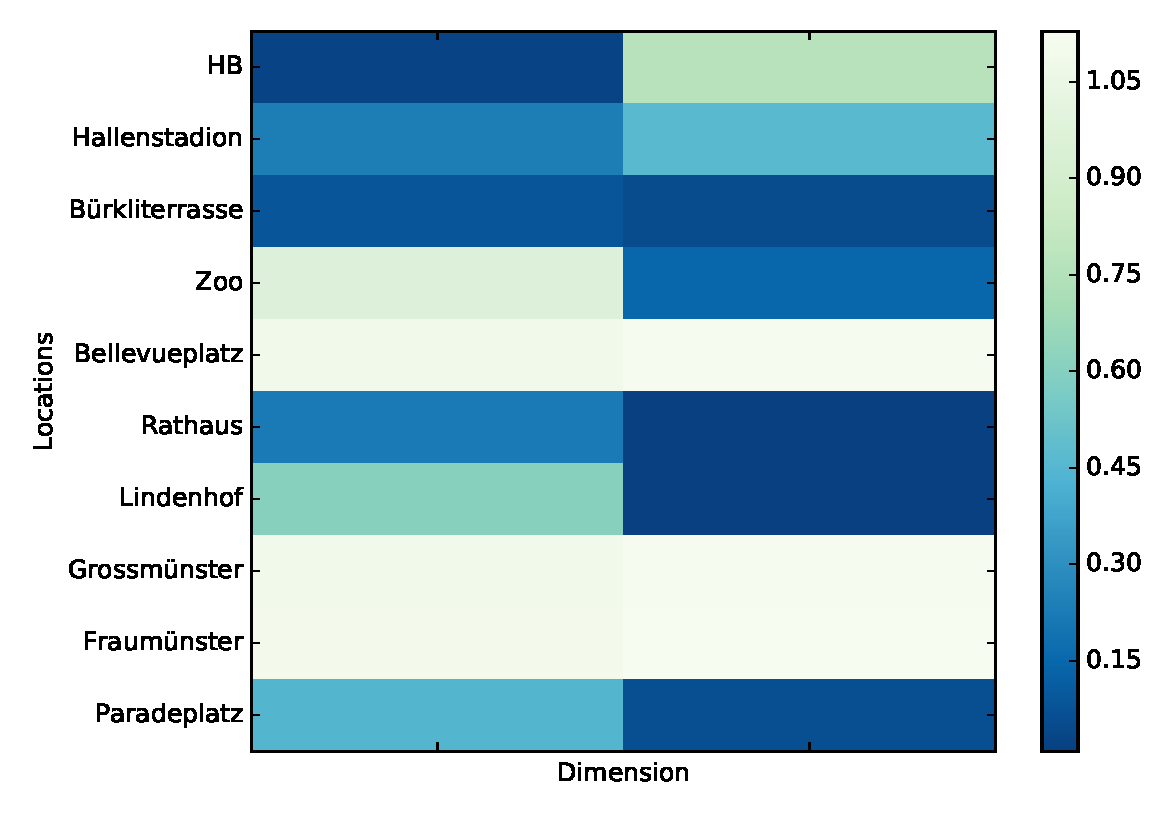
\includegraphics[width=0.7\textwidth]{submodular_weights_d_2}
    \end{figure}
  \end{frame}
  
  \begin{frame}{Diversity Encoding ($d=5$)}
    \begin{figure}
      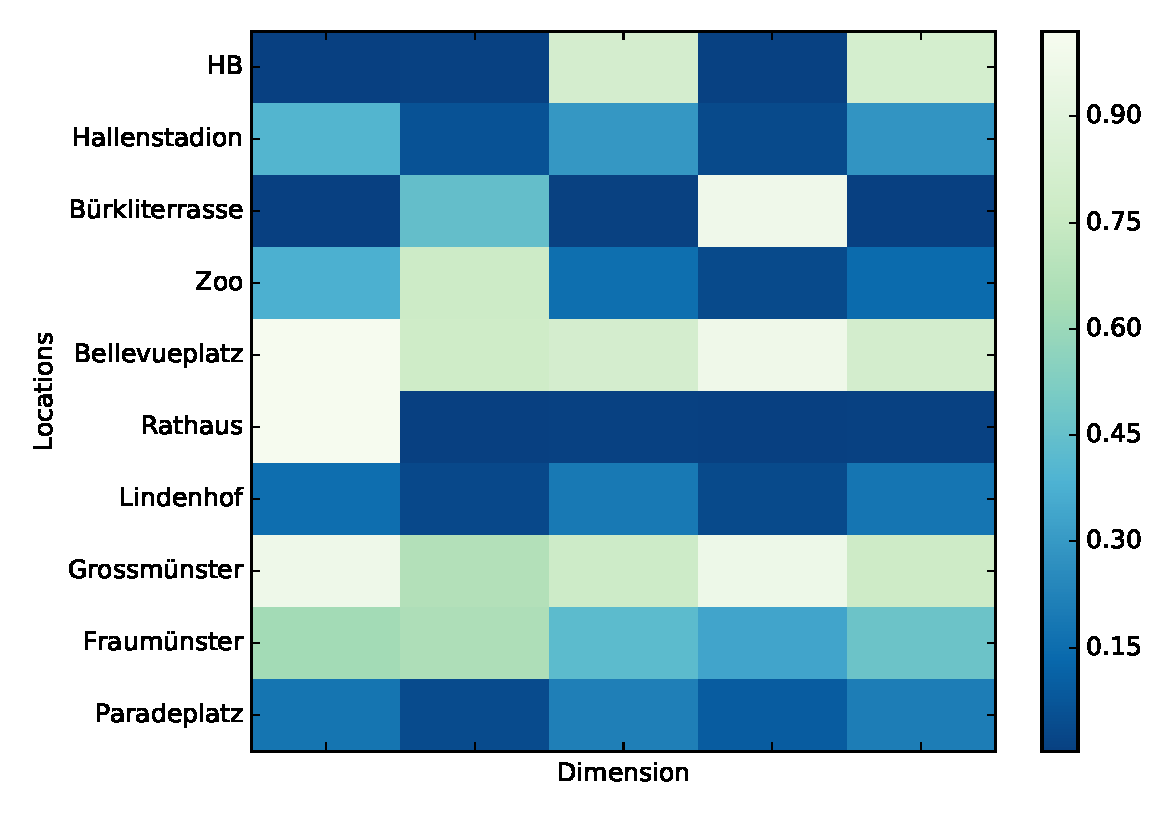
\includegraphics[width=0.7\textwidth]{submodular_weights_d_5}
    \end{figure}
  \end{frame}
  
  \begin{frame}{Diversity Encoding ($d=10$)}
    \begin{figure}
      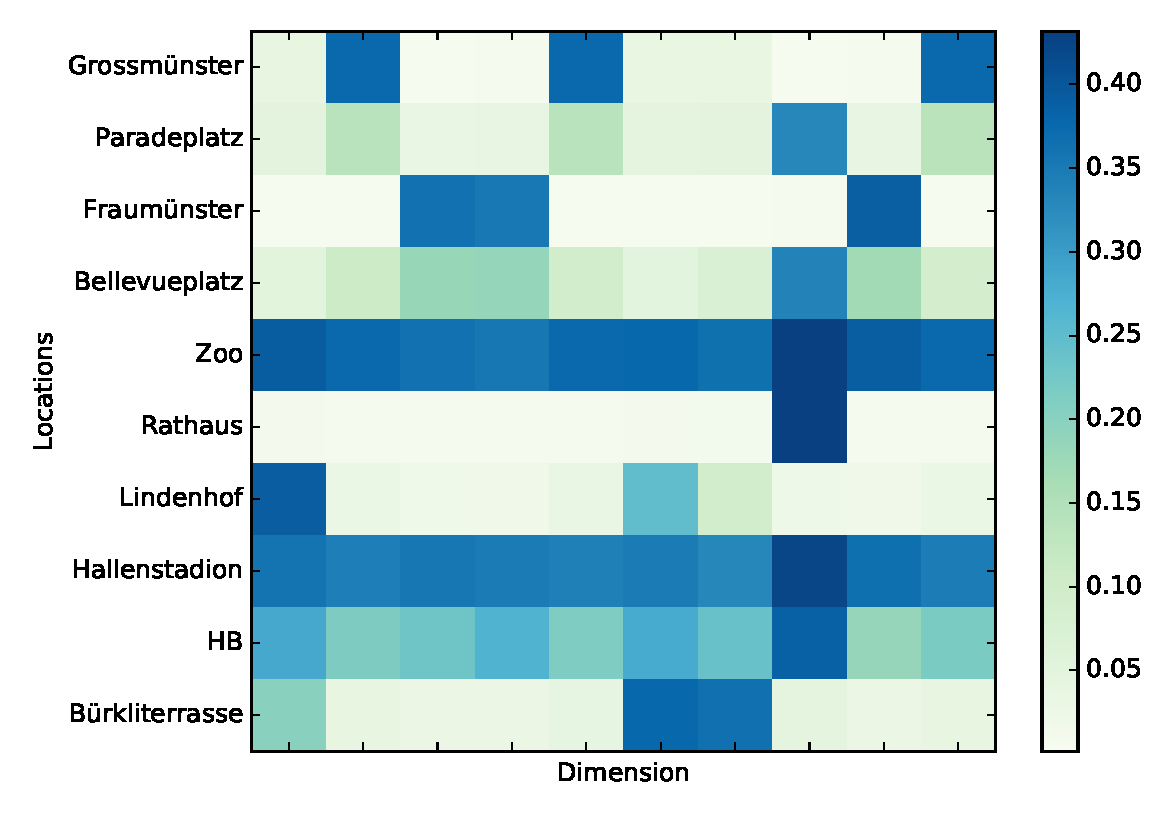
\includegraphics[width=0.7\textwidth]{submodular_weights_d_10}
    \end{figure}
  \end{frame}
  
  \section{New Baselines}
  
  \begin{frame}{Proximity Model}
    Assuming a partial ordered sequence $S$ of length $k$ for geo-located items, the model defines a score $Q(i \mid S)$.
    \begin{equation}
      \forall{i \notin S}: Q(i \mid S) = \frac{1}{d(i, s_{k})}
    \end{equation}
    Where $d(a,b)$ is the great-circle distance between items $a$ and $b$, and $s_{k}$ is the $k_{th}$ element of the sequence.

    The set of items to suggest for $S$ is ordered descendingly according to $Q(i|S)$.
  \end{frame}
  
  \begin{frame}{Markov Model}
    As proposed by \cite{Kurashima2010}. The probability of visiting a location given a location history $S = \langle s_{1} \dots s_{k} \rangle$ can be modeled as:
    
    \begin{equation}
      P(s_{k+1} = i \mid s_{1} \dots s_{k}) = P(s_{k+1} = i \mid s_{k})
    \end{equation}
    
    Which can be estimated with maximum likelihood from the data as:
    
    \begin{equation}
      P(s_{k+1} = i \mid s_{k}) = \frac{N(l_{t+1} = i, l_{t} = s_{k})}{N(l_{t} = s_{k})}
    \end{equation}
    
    Where $N(l_{t+1} = i, l_{t} = s_{k})$ is the number of times that $i$ was visited immediately after $s_{k}$, and $N(l_{t} = s_{k})$ is the number of times that $s_{k}$ was visited.
    
    The set of items to suggest for $S$ is ordered descendingly according to $P(i \mid S)$.
  \end{frame}
  
  \begin{frame}{Results}
    The new baseline models were trained on the data and the same 10-fold evaluation was performed, the results are:
    \begin{table}
      \begin{tabularx}{0.7\textwidth}{X|c|c|c|c}
        Model         & $Acc$ & $\sigma_{Acc}$ & $MRR$ & $\sigma_{MRR}$ \\
        \hline
        Modular & 16.42 & 2.42 & 44.47 & 1.40 \\
        FLID ($d=10$) & 26.32 & 3.35 & 50.00 & 1.92 \\
        Markov & 30.18 & 2.59 & 53.41 & 1.76 \\
        Proximity & 11.61 & 0.99 & 33.99 & 0.99 \\
      \end{tabularx}
    \end{table}
  \end{frame}
  
  \section{Including Features}
  
  \begin{frame}{Definitions}
    \begin{description}
      \item[$\bm{V}$] The set of locations, with cardinality $N = \lvert \bm{V} \rvert$.
      \item[$M$] The number of features that define each location.
      \item[$L$] The number of latent concepts.
      \item[$\bm{X}$] The feature matrix for the locations, $\bm{X} \in \mathbb{R}^{N \times M}$.
      \item[$\bm{a}$] The vector that defines the utility weight for each feature, $\bm{a} \in \mathbb{R}^{M}$.
      \item[$\bm{B}$] The matrix that defines the contribution of each feature to a latent diversity concept, $\bm{B} \in \mathbb{R}^{M \times L}$.
    \end{description}
  \end{frame}
  
  \begin{frame}{FLID with Features}
    The FLID model with features is defined by:
    
    \begin{equation}
      P(S \mid \bm{a}, \bm{B}) = \frac{1}{Z} \exp{\left(\sum_{i \in S}{\bm{x}_{i}\bm{a}} + \sum_{l = 1}^{L}{\left( \max_{i \in S}{\bm{x}_{i}\bm{b}_{l}} - \sum_{i \in S}{\bm{x}_{i}\bm{b}_{l}} \right)} \right)}
    \end{equation}
    
    Where $\bm{x}_{i}$ is the $i$-th row of $\bm{X}$, and $\bm{b}_{l}$ is the $l$-th column of $\bm{B}$. This is analog to the previous model if we define $\bm{u}$ and $\bm{W}$ as:
    
    \begin{eqnarray*}
       \bm{u} = \bm{X}\bm{a} \\
       \bm{W} = \bm{X}\bm{B}
    \end{eqnarray*}
  \end{frame}
  
  \begin{frame}{NCE learning}
    To modify the NCE learning algorithm, it is just necessary to change the definition of the sub-gradient as follows:
    
    \begin{eqnarray}
      \left(\nabla_{\bm{a}} \log{\frac{1}{\hat{Z}} \tilde{P}\left(S \mid \bm{a},\bm{B} \right)}\right)_{m} = \sum_{i \in S}{x_{i,m}} \\
      \left(\nabla_{\bm{B}} \log{\frac{1}{\hat{Z}} \tilde{P}\left(S \mid \bm{a},\bm{B} \right)}\right)_{m, l} = x_{i^{*},m} - \sum_{i \in S}{x_{i,m}} \label{eq:gradient_b}
    \end{eqnarray}
    
    Where $x_{i^{*},m}$ in equation \ref{eq:gradient_b} is:
    
    \begin{equation*}
      i^{*} = \argmax_{i \in S} \bm{x}_{i} \bm{b}_{l}
    \end{equation*} 
    
    The subgradient for $\hat{Z}$ is unchanged.
    
  \end{frame}
  
  \bibliographystyle{apalike}
  \section*{References}
  \begin{frame}{References}
    \bibliography{../references}{}
  \end{frame}

\end{document}
